\documentclass[12pt,letterpaper]{amsart}
\setlength{\oddsidemargin}{.0in}
\setlength{\evensidemargin}{.0in}
\setlength{\textwidth}{6.5in}
\setlength{\topmargin}{-.3in}
\setlength{\headsep}{.20in}
\setlength{\textheight}{9.in}
\renewcommand{\baselinestretch}{1.4}
\usepackage[leqno]{amsmath}
\usepackage{amsfonts}
\usepackage{amssymb}
\usepackage{amsthm}
\usepackage{amssymb}
\usepackage[all]{xy}
\usepackage{graphicx}


%Here are some user-defined notations
\newcommand{\RR}{\mathbf R}
\newcommand{\CC}{\mathbf C}
\newcommand{\ZZ}{\mathbf Z}
\newcommand{\ZZn}[1]{\ZZ/{#1}\ZZ}
\newcommand{\QQ}{\mathbf Q}
\newcommand{\rr}{\mathbb R}
\newcommand{\cc}{\mathbb C}
\newcommand{\zz}{\mathbb Z}
\newcommand{\zzn}[1]{\zz/{#1}\zz}
\newcommand{\qq}{\mathbb Q}
\newcommand{\calM}{\mathcal M}
\newcommand{\latex}{\LaTeX}
\newcommand{\tex}{\TeX}
\newcommand{\sm}{\setminus} 


%improving spacing in tables (space above and below characters in a row)
\newcommand{\tfix}{\rule{0pt}{2.6ex}}
\newcommand{\bfix}{\rule[-1.2ex]{0pt}{0pt}}


%Here are commands with variable inputs 
\newcommand{\intf}[1]{\int_a^b{#1}\,dx}
\newcommand{\intfb}[3]{\int_{#1}^{#2}{#3}\,dx}
\newcommand{\pln}[1]{$\sm${\tt #1}}
\newcommand{\bgn}[1]{$\tt {\sm}begin\{#1\}$}
\newcommand{\nd}[1]{$\tt {\sm}end\{#1\}$}
\newcommand{\marginalfootnote}[1]{%
        \footnote{#1}
        \marginpar[\hfill{\sf\thefootnote}]{{\sf\thefootnote}}}
\newcommand{\edit}[1]{\marginalfootnote{#1}}


%Here are some user-defined operators
\newcommand{\Tr}{\operatorname {Tr}}
\newcommand{\GL}{\operatorname {GL}}
\newcommand{\SL}{\operatorname {SL}}
\newcommand{\Prob}{\operatorname {Prob}}
\newcommand{\re}{\operatorname {Re}}
\newcommand{\im}{\operatorname {Im}}


%These commands deal with theorem-like environments (i.e., italic)
\theoremstyle{plain}
\newtheorem{theorem}{Theorem}[section]
\newtheorem{corollary}[theorem]{Corollary}
\newtheorem{lemma}[theorem]{Lemma}
\newtheorem{conjecture}[theorem]{Conjecture}

%These deal with definition-like environments (i.e., non-italic)
\theoremstyle{definition}
\newtheorem{definition}[theorem]{Definition}
\newtheorem{example}[theorem]{Example}
\newtheorem{remark}[theorem]{Remark}

%This numbers equations by section
\numberwithin{equation}{section}


\begin{document}



\title{Math 3094:  Mathematics for Machine Learning \\(Spring 2023)}

\maketitle

\thispagestyle{empty}

{\bf Machine Learning} is a ``hot topic'' that brings together ideas from computer science, statistics, and mathematics to
extract structures from large data sets. As a branch of artificial intelligence, it has applications in building automated systems, identifying patterns and making decisions. Some typical problems in machine learning include image
recognition, fraud detection and extracting meaning from text.

Machine Learning uses mathematics as its basic language and main resource of important techniques. In order to exploit the immense possibilities of Machine Learning, a thorough  mathematical understanding of many of these techniques is necessary.

In this course we will discuss the mathematical foundations of key algorithms in Machine Learning, and, through lab projects, apply these algorithms to some “real world” data. This course will incorporate computer work in Python. Necessary programming skills will be taught as part of the course.

\bigskip 

{\bf Prerequisites}:  Multivariable Calculus (2110) and Linear Algebra (2210). Contact the instructor (Jeremy Teitelbaum, at jeremy.teitelbaum@uconn.edu) for a permission number.

\bigskip

{\bf Class Time}: Tu/Th 9:30 am - 10:45 am

\bigskip


\begin{figure}[ht]
   \center
   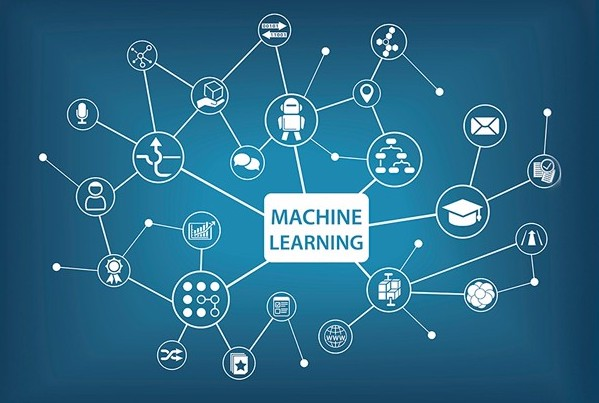
\includegraphics[scale=.35]{ml.jpeg} \hspace{1cm}      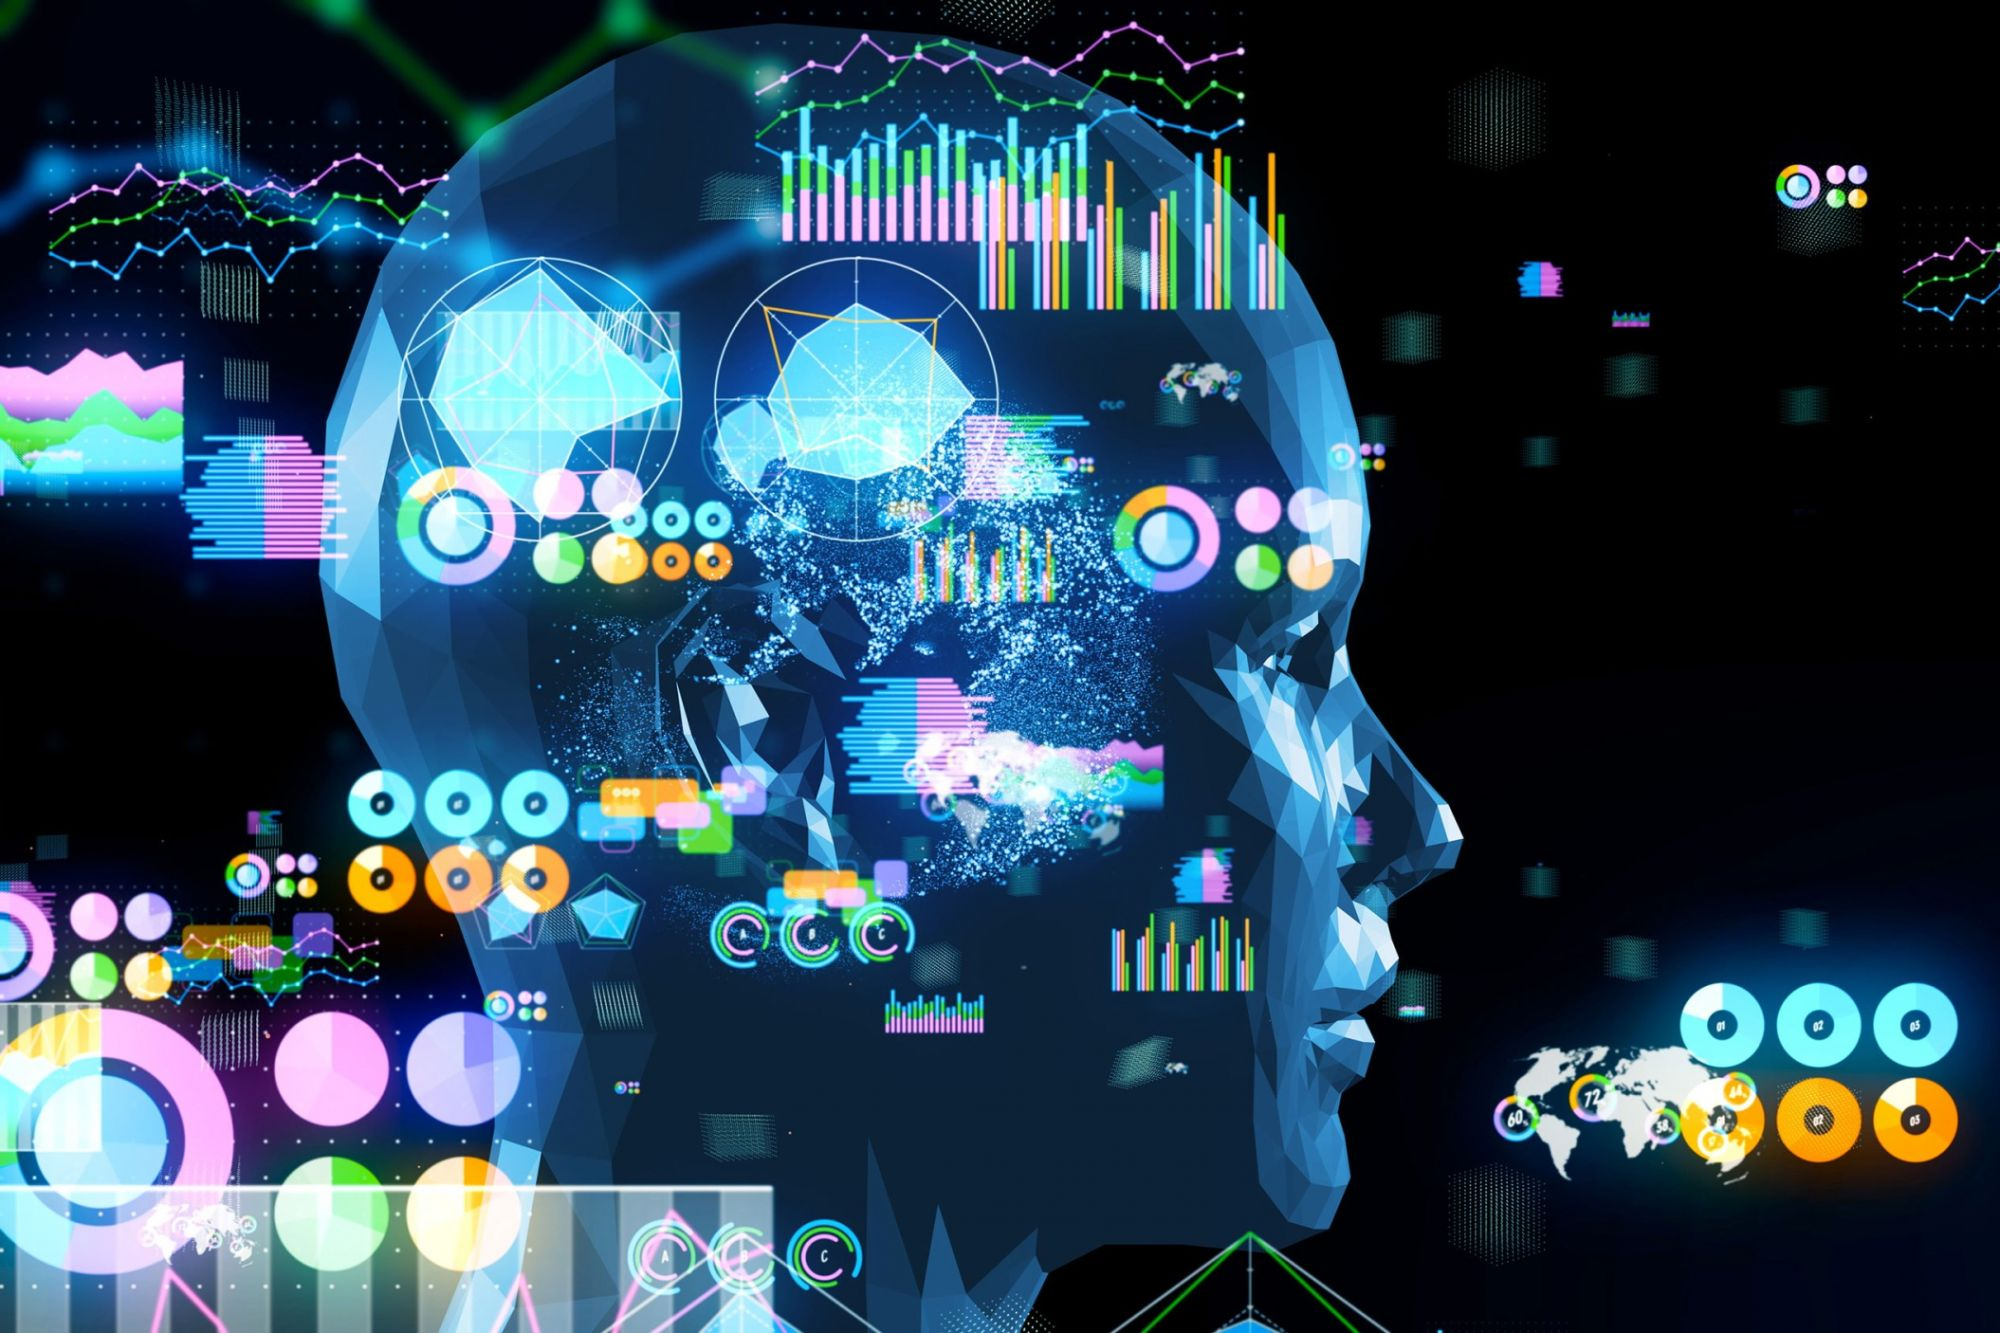
\includegraphics[scale=.105]{ml-2.jpeg}  
\end{figure}



{\bf Questions?} Email the instructor, Jeremy Teitelbaum (jeremy.teitelbaum@uconn.edu).

\end{document}








